\documentclass[12pt]{beamer}
\usepackage[english, russian]{babel}
\usepackage[utf8]{inputenc}
\usepackage{graphicx}
\usepackage{hyperref}
\usepackage{minted}
\usepackage{amsmath}
\usepackage{amssymb}

\hypersetup{
    colorlinks=true,
    linkcolor=blue,      
    urlcolor=cyan,
}

\graphicspath{ {./assets/} }

\usetheme{Madrid}

\title{Задача о размещении}
\subtitle{с ограничениями на мощности производства}
\author{Карабалин Руслан}
\date{21 декабря 2024 г.}

\begin{document}
	
	\begin{frame}
		\titlepage
	\end{frame}

    \begin{frame}
        \frametitle{Содержание}

        \begin{itemize}
            \item Постановка задачи;
            \item Математическая модель;
            \item Алгоритмы решения;
            \item Пример задачи с решением;
            \item Выводы.
        \end{itemize}

    \end{frame}

    \begin{frame}
        \frametitle{Постановка задачи}

        Имеется $\boldsymbol{I}$ возможных пунктов размещения предприятий
        по производству некоторого однородного продукта.
        Велечина $\boldsymbol{c_{i}}$ задает стоимость открытия предприятия
        в пункте $\boldsymbol{i}$, а величина $\boldsymbol{V_{i}}$ определяет максимально
        возможный объем производства в данном пункте.
        Перечень потребителей задается множеством $\boldsymbol{J}$.
        Для каждой пары $\boldsymbol{(i, j)}$ известа велечина $\boldsymbol{g_{ij}}$
        затрат на производство и доставку продукции потребителю,
        а также велечина $\boldsymbol{p_{ij}}$ - объем продукции $\boldsymbol{i}$-го предприятия,
        необходимый для удовлетворения потребностей
        $\boldsymbol{j}$-го потребителя.
        
    \end{frame}

    \begin{frame}
        \frametitle{Математическая модель}
    
        \textbf{Дано:}
        \begin{itemize}
            \item $I$      --- множество мест размещения предприятий;
            \item $J$      --- множество потребителей, которых нужно обслужить;
            \item $c_i$    --- стоимость размещения объекта в месте $i \in I$;
            \item $V_{i}$  --- максимальный объем производства в пункте $i \in I$;
            \item $g_{ij}$ --- стоимость обслуживания объекта $j \in J$ из места $i \in I$;
            \item $p_{ij}$ --- объем продукции $i$-го предприятия, необходимый для удовлетворения потребностей $j$-го потребителя.
        \end{itemize}

        \textbf{Переменные:}
        \begin{itemize}
            \item $y_i \in \{0, 1\}$    --- $1$, если предприятие $i \in I$ открыто, и $0$ в противном случае;
            \item $x_{ij} \in \{0, 1\}$ --- $1$, если потребитель $j \in J$ обслуживается из предприятия $i \in I$, и $0$ в противном случае.
        \end{itemize}
    
    \end{frame}

    \begin{frame}
        \frametitle{Математическая модель}
    
        \textbf{Целевая функция:}
        \begin{equation}
            F(x) = \sum_{i \in I} c_i y_i + \sum_{i \in I} \sum_{j \in J} g_{ij} x_{ij} \to \min
        \end{equation}

        \textbf{Ограничения:}
        \begin{equation}
            \sum_{i \in I} x_{ij} = 1, \quad \forall j \in J
        \end{equation}
        \begin{equation}
            \sum_{j \in J} p_{ij} x_{ij} \leq V_{i} y_{i}, \quad \forall i \in I
        \end{equation}
        \begin{equation}
            x_{ij}, y_i \in \{0, 1\}, \quad i \in I, j \in J
        \end{equation}
    
    \end{frame}

    \begin{frame}
        \frametitle{Алгоритмы решений}
    
        \begin{columns}
            \begin{column}{0.5\textwidth}
                \begin{itemize}
                    \item Метод ветвей и границ;
                    \item Метод отсечений;
                    \item Жадный алгоритм.
                \end{itemize}
            \end{column}
            \begin{column}{0.5\textwidth}
                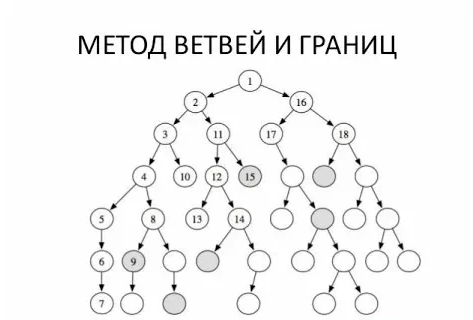
\includegraphics[width=1\textwidth]{vetvi.png}
            \end{column}
        \end{columns}
    
    \end{frame}

    \begin{frame}
        \frametitle{Пример задачи}
    
        \begin{itemize}
            \item Дано множество возможных мест размещения \( I = \{A, B, C\} \) и множество объектов (клиентов) \( J = \{1, 2, 3\} \).
            \item Стоимость размещения производства в местах: $c_A = 100, \quad c_B = 120, \quad c_C = 150.$
            \item Производственная мощность каждого места: $u_A = 50, \quad u_B = 60, \quad u_C = 40.$
            \item Потребности объектов: $b_1 = 30, \quad b_2 = 20, \quad b_3 = 40.$
            \item Стоимость доставки единицы продукции от мест размещения к объектам:
            \[
            d_{ij} = 
            \begin{bmatrix}
            10 & 15 & 20 \\
            20 & 10 & 25 \\
            15 & 20 & 10
            \end{bmatrix}
            \]
        \end{itemize}
    
    \end{frame}

    \begin{frame}
        \frametitle{Пример решения}
    
        \begin{itemize}
            \item Рассмотрим \( x_A = 1, x_B = 1, x_C = 0 \), что означает размещение производств только в \( A \) и \( B \).
            \item Распределение доставки:
            \[
            y_{A1} = 30, \quad y_{B2} = 20, \quad y_{B3} = 40.
            \]
            \item Проверим мощности:
            \[
            \text{Для } A: \quad y_{A1} = 30 \leq 50, \quad \text{выполнено.}
            \]
            \[
            \text{Для } B: \quad y_{B2} + y_{B3} = 20 + 40 = 60 \leq 60, \quad \text{выполнено.}
            \]
        \end{itemize}
    
    \end{frame}

    \begin{frame}
        \frametitle{Результат}
    
        \textbf{Расчёт затрат:}

        $$F = 100x_A + 120x_B + 10y_{A1} + 10y_{B2} + 25y_{B3}$$
        $$= 100 + 120 + 10 \cdot 30 + 10 \cdot 20 + 25 \cdot 40 = 1650$$

        \begin{block}{Ответ:}
            \begin{itemize}
                \item Размещать производства в точках \( A \) и \( B \).
                \item Распределение продукции:
                \[
                y_{A1} = 30, \quad y_{B2} = 20, \quad y_{B3} = 40.
                \]
                \item Общие затраты: \( F = 1650 \).
            \end{itemize}    
        \end{block}

    \end{frame}

    \begin{frame}
        \frametitle{Выводы}
    
        \begin{itemize}
            \item Задача о размещении с ограничениями на мощности производства позволяет минимизировать затраты на открытие производств и доставку продукции, учитывая ограничения на производственные мощности;
            \item Применение методов оптимизации, таких как метод ветвей и границ или метод отсечений, позволяет найти точное решение для небольших задач;
            \item Для крупных задач эффективны приближённые и эвристические методы, такие как жадный алгоритм или генетические алгоритмы;
            \item Модель может быть адаптирована для различных прикладных задач, например, логистики, планирования производств или размещения инфраструктурных объектов.
        \end{itemize}
    
    \end{frame}

    \begin{frame}
        \frametitle{Литература}

        \begin{itemize}
            \item Алексеева Е. В. Построение математических моделей целочисленного линейного программирования. Примеры и задачи: Учеб. пособие / Е. В. Алексеева. - Новосибирск: НГУ, 2012. - 131 с.
            \item Задачи размещения: тестовые данные для решения задачи размещения предприятий с фиксированными затратами [Электронный ресурс] / Институт математики им. С. Л. Соболева СО РАН. \url{http://old.math.nsc.ru/AP/benchmarks/CFLP/cflp.html}
        \end{itemize}

    \end{frame}
	
\end{document}
